\section{Case Study}
\label{sec:casestudy}
A design and fabrication workshop was organized to examine the feasibility of our system with a specific design target and a location.
We selected a public community house where people in the community share the space and regularly use the facility.
Participants of the workshop were selected among them, who were four children (aged 4, 7, 9, and 10) and two parents (Figure~\ref{fig:workshop}).
We specifically selected children with this range of age as non-experts without experiences in computational design or digital fabrication, also for observing the clarity and attractiveness of the game.

The entire workshop was filmed and summarized in the supplementary video material.
Prior to the workshop, we have adjusted the weights in Equation \ref{eq:score} manually to ensure that the feasibility of layouts is correlating to the scores (see Figure \ref{fig:testlayouts}). 
Through adjusting the game setting, we have built six target frames.

The goal for the participants was to contribute to an ongoing design and fabrication process of screen wall (2000 $mm$ $\times$ 900 $mm$) consisting of eight rectangles (500 $mm$ $\times$ 450 $mm$).
Six frames were already designed and built, thus the rest two frames were prioritized for them to design and fabricate in this workshop.

Participants were informed about the goal of the workshop, and each process was introduced by experienced tutors.
The processes were from collecting and fixing the branches on a plate, scanning the plate, complete designs by playing the game, and assembly after CNC milling.

\begin{figure}[ht]
  \begin{center}
    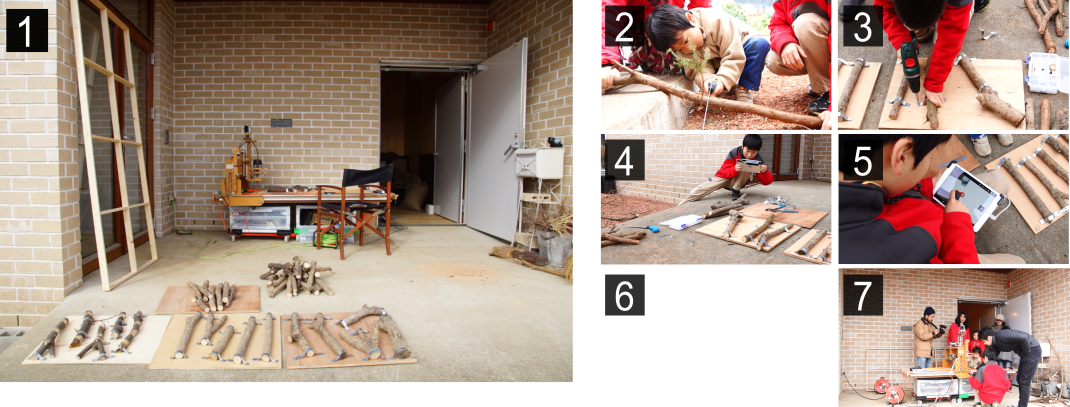
\includegraphics[width = 0.4\paperwidth]{images/fabrication/workshop_setup.png}
    \caption{An overview of the workshop. 1. the overview of the space. 2. collect branches. 3. cut in certain lengths 4. attach on a plate 5. scan the plate 6. play the game 7. CNC milling.}
    \label{fig:workshop}
  \end{center}
\end{figure}

\subsection{Preparations and User Experiences}
\subsubsection*{System and Hardware}
We used two iPad minis with iSense depth cameras attached for scanning branches, and a 3 axis CNC milling router with a 6 mm diameter milling bit.
We used a laptop PC for running \textit{Branch Importer} and \textit{G-Code generator}, as well as operating the milling machine.
The scan area of iSense camera is 500 $mm$ $\times$ 500 $mm$, and the milling machine's stroke length along z-axis is 70 $mm$, which provide geometric constraints for available branch sizes.
\textit{BranchConnect} was hosted at \textit{Heroku} cloud server \footnote{Heroku is a platform as a service (PaaS) that enables developers to build, run, and operate applications entirely in the cloud. \url{https://www.heroku.com/}},
and we used \textit{MongoDB} \footnote{MongoDB is a free and open-source cross-platform document-oriented database program. \url{https://www.mongodb.com/}} as a cloud database.

\subsubsection*{Preparations}
The participants were asked to collect branches with 20 - 100 $mm$ in diameter.
The lower bound was for the milling bit size, and the upper bound was for the limited length of z-stroke of the CNC router.
The collected branches were cut in arbitrary lengths, not longer than 500 $mm$ due to the limit of scanning area. 
As our game system and fabrication process take 3D branch shapes as 2D contours (with limited use of point cloud), these constraints were benefitial for the system by filtering out branches with large 3D twists.
The diameter and length constraints worked as guidelines for participants rather than restricting finding and cutting arbitrary branches.
The number of available branches per plate was different depending on branch sizes.
Within the feasible diameter of branches and the plate size, the number of available branches was  most up to six (see Figure \ref{fig:scannedplates}).

After cutting branches in certain lengths, participants fixed branches on plates by thin metal fixtures with screw holes.
After an instruction, participants successfully fixed branches by themselves.
%It was straightforward for them to firmly fix branches so that they are not moved during milling process.
%These fixture points are counted as invalid points in the game where joinery points can not be generated.
They built two plates with three and five branches fixed on each plate.

After fixing branches on plates, we asked participants to scan them prepare feasible mesh model on iSence application running on iPad mini.
Thanks to the intuitive interface of iSense, participants practiced several scans and successfully scanned models without problem.
After obtaining mesh models, tutors imported models from iPads to a laptop and uploaded them to the database by \textit{Branch Importer}.



\subsubsection*{User Experiences}
%After models were uploaded to the server, participants could that their plates are added in the selectable branch plates with their names and locations.
As for more general user experiences with the game, see Section \ref{sec:game} as well as the video material.
%Users could access to the start page by PC and mobile devices.
In this section, we describe more specific user experiences and feedback from participants.

%We prepared both options and let participants choose a device.
All participants used iPads for navigating pages and playing the game.
They had difficulties with mobile touch interface, such as rotation and flipping operation by gestures.
We had several requests from participants regarding the game interface but also related to the workshop organization. Several participants requested to allow multiple branch plates for designing a frame, or even remove the target frame and let them freely design with branches.
Also a participant who gave up the game with iPad requested additional buttons for mobile touch interface, such as to keep an active branch selected.
The participant with four years old failed to complete the game.
He insisted on accepting his design to be fabricated 
Similarly, a branch plate made by a participant had only three branches, which was not enough to fulfill bridging target points, however, the participant insisted on accepting it in the selection.
%We took them as positive inputs to validate our participatory (architectural) design approach.
%A user is firstly directed to a start page and asked to submit a user name.
%Secondly, the user is navigated to target frame selection page, and asked to pick one out of eight frames.
%Each frame has different target points.
%The interface also shows the completed branch organizations within each target frame.
%If there are multiple designs, three designs with highest scores are displayed.
%The user can change the currently displayed design by clicking within each frame and choose either starting their design from scratch, or select the design and improve it.
%After selecting a target frame, the user goes to branch selection page, displaying 15 plates when the workshop was held.
%In this page, they saw the plates made by themselves on the page, as well as their names on the plate.
%The user can select the same plate for designing other target frames.
%By clicking a displayed branch plate, the user is navigated to the game interface.
%After completing to bridge all the target points, the design is automatically uploaded to the database, but the use can continue to design.


\subsubsection*{Global Design Consensus and Fabrication} 
As the target frame selection page could display all layout designs, we could get an overview of design options.
The layout designs were displayed as score descending order with limited numbers (three top highest scores for each target frame), we could find feasible layout designs easily with mostly all the target points were bridged.
As participants were excited by seeing their branches and designs, we took two invalid layout designs and one plate which did not have enough branches for the global design.
%
%\subsubsection*{Fabrication}
After selecting layouts, an experienced tutor operates \textit{G-Code Generator} as well as the CNC router.
Participants were asked to assembly branches after joineries were milled.

\subsection{Results}


The entire workshop took 4.6 hours to complete the whole process, including introduction, moving, and pauses.
Table below shows durations of each task.

\begin{center}
  \begin{tabulary}{\columnwidth}{ |l||C|C| }
    \hline
    Task & Duration (hour) & Fraction ($\%$) \\
    \hline
    Introduction                  & 0.3 & 6.5  \\
    Collecting branches           & 0.6 & 13.0  \\
    Preparing plates              & 0.8 & 17.4  \\
    Preparing models              & 0.3 & 6.5  \\
    Uploading models              & 0.2 & 4.3 \\
    Designing by the game         & 0.5 & 10.8 \\
    Inspecting models             & 0.2 & 4.3 \\
    CNC milling                   & 0.5 & 10.8\\
    Assembling                    & 0.2 & 4.3 \\
    Moving, pauses               & 1.0 & 21.7 \\
    \hline
    In total                      & 4.6   & 100 \\
    \hline
  \end{tabulary}
  \label{tab:timing}
\end{center}



\subsubsection*{Model Acquisition}
Each scanning and re-touching took 2-3 minutes, and 30 seconds for generating data by \textit{Branch Importer}.
Including the prepared panels previously, we scanned 15 plates in total, 75 branches, and 35.3m of total length including sub-branches.
We got 59 branches with a single skeleton, 16 branches with multiple skeletons for grafting.
The result is shown in Figure \ref{fig:scannedplates}.

\begin{figure}[ht]
  \begin{center}
    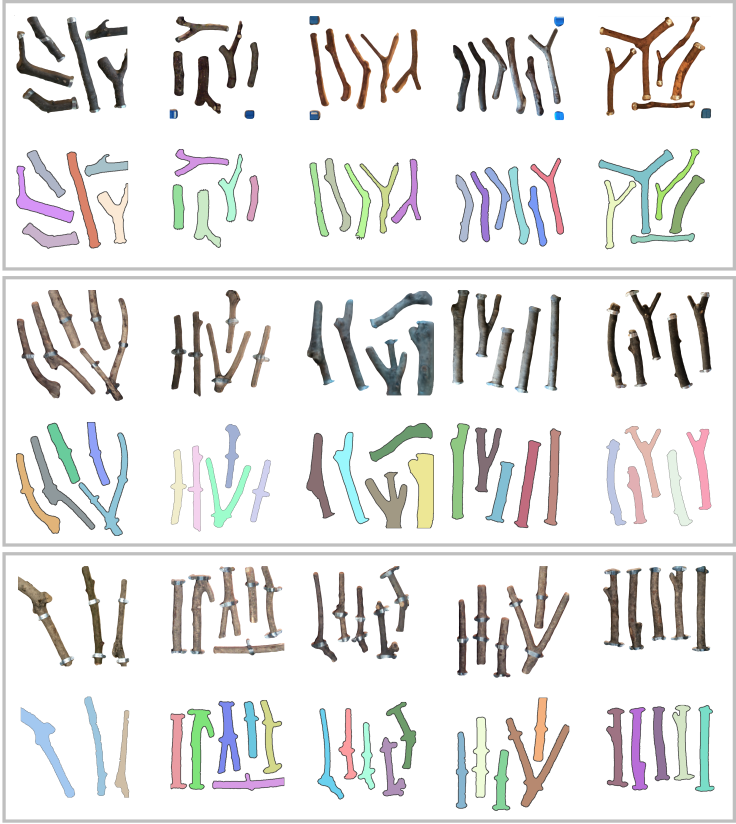
\includegraphics[width = 0.4\paperwidth]{images/fabrication/all_plates.png}
    \caption{An overview of all the 15 scanned plates for the construction of the fence. Top raw of each set shows ortho-top views of scanned mesh models, and the bottom raw is the recognized branches with randomly assigned colors. The red-lined rectangles indicate the plates built by participants in the workshop.}
    \label{fig:scannedplates}
  \end{center}
\end{figure}


\subsubsection*{Design with the Game}
Figure \ref{fig:testlayouts} shows 32 example layouts with scores.
We set the weights in Equation \ref{eq:score} as shown in Table below.

\begin{center}
	\begin{tabulary}{\columnwidth}{ |1|C|C|C|C|C|C|    }
		\hline
		weigths & $w_1$ & $w_2$ & $w_3$ & $w_4$ & $w_5$ \\
		\hline
		our setting & 100 & -100 & -1000 & 500 & -5\\
		\hline
	\end{tabulary}
	\label{tab:weights}
\end{center}

\begin{figure}[ht]
	\begin{center}
		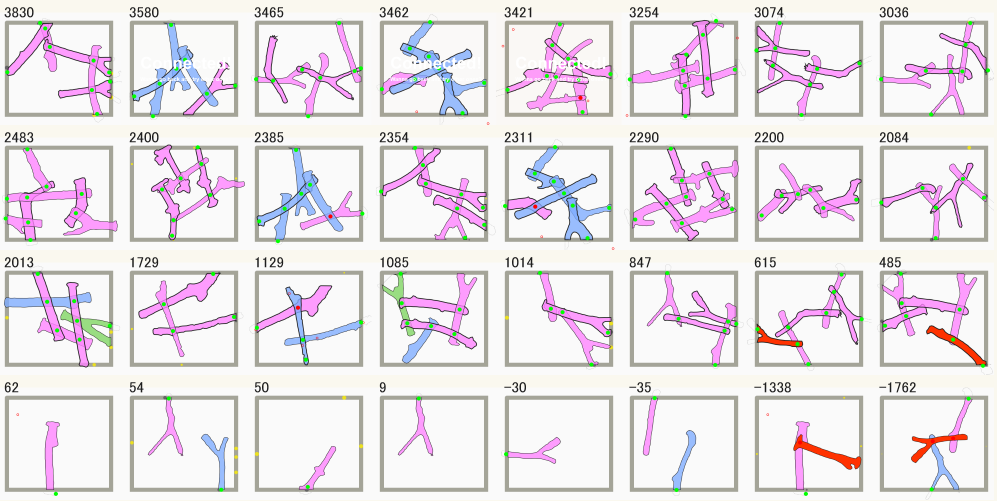
\includegraphics[width = 0.4\paperwidth]{images/fabrication/designs_score.png}
		\caption{Example layouts by authors in score-descending order. The highest score is top-left and the lowest score is bottom-right.}
		\label{fig:testlayouts}
	\end{center}
\end{figure}

One participant switched to play by a PC for more precise control due to the problem.
Interestingly, all the participants chose to develop their own designs from the scratch, although they had instruction about the "continue existing designs".

We set 30 minutes for playing the game, and eight layout designs were given by participants.
Two frames were completed per participants and two participants completed the whole eight target frames.
The average score was xxx, and average playing duration was xxx to complete each target frame. \todo{recheck the numbers by server}


\subsubsection*{Fabrication}
%We did not have major problems for converting designs to G-Code milling paths as we encountered major issues regarding the fabrication before the workshop, which are reported in this section.

%We encountered problem was the accuracy of acquired contours.
We observed most of scanned models had occluded regions between plates and branches, which create interpolated faces during solidifying process, resulting in outwardly offsetted contours. \todo{check offsetted correct english} After milling was finished and when branches were assembled, six pairs of branches were loosely connected because the calculated contours were 2-3 $mm$ eroded than the actual sizes.
We avoided this problem by trimming branches from 2-5 $mm$ higher than the plate surface.
After this operation, the rest of connections were tightly connected. \\

We also observed that many milling paths were 5-10 $mm$ off from the center of planned joints.
Multiple reasons could be considered as reasons such as,

\begin{itemize}
  \item{deformation of mechanical parts of the CNC router}
  \item{not dense resolution of acquired contours of branches}
  \item{misaligned orientation of the plate compared to the scanned model}
\end{itemize}

To avoid the misalignments, we modified the \textit{G-Code Generator} so that an operator can freely adjust the absolute origin of the generated milling paths.
The origin was usually set with around the center of the plate.
After this modification, the misalignment from joint center was reduced with 5 $mm$ off at the maximum misalignment.
Branches could absorb 3-5 $mm$ misaligned joint positions due to the elasticity of branches, and solidifying the structure with residual stresses from misalignments.
% The misaligned joint positions worked as post-tensions, solidifying the structure.
% We assume that this is only applicable when an applied bending moment and cut surface at a joint is orthogonal or not too much off from orthogonal. \todo{this sentence}




